\section{Case Study}
\label{sec:Evaluation.CaseStudy}

This section presents a case study that uses combinations of languages of the Epsilon platform to implement a number of model management tasks. The scenario and requirements of the case study have been defined by the organizers of the Model Driven Development Tools Implementers Forum (MDD-TIF) \cite{MDDTIF} to enable a comparison of several different MDE tools using a common basis.

\subsection{Scenario}

The following case study description has been taken as-is from the MDD-TIF web-site \cite{MDDTIF}.

\subsubsection{Abstract}
Digital television allows interactive content to accompany standard broadcasts. The development of bespoke interactive content is expensive. You are to design a system that will allow the non-technical producers of television programmes to build interactive content from a set of high-level building blocks.
In effect, you will create a modelling language (metamodel, rules and symbols), a tool supporting it, and a generator.

\subsubsection{Background}
Digital television is becoming increasingly popular in the UK. In addition to providing higher quality video and increased channel capacity, it allows interactive content to accompany standard broadcasts. Interactive applications have been used to enhance traditional broadcasts in many ways:

\begin{itemize}
	\item Viewers can play along with quizzes (Figure \ref{fig:MDDTIFFigure1}).
	\item Viewers can choose different camera angles during sporting events
	\item Viewers can take part in discussions and comment on events though message boards.
	\item Viewers can remind themselves of the important developments in a drama's plot (Figure \ref{fig:MDDTIFFigure2}).
\end{itemize}

\begin{figure}
	\centering
		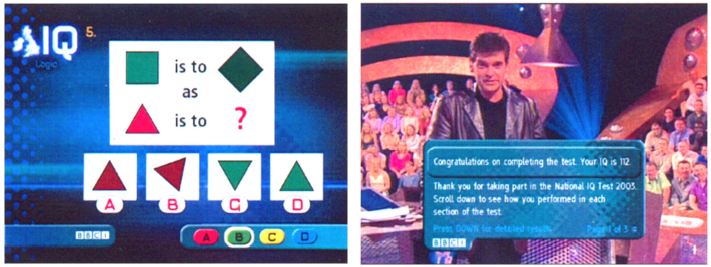
\includegraphics[width=1\textwidth]{images/MDDTIFFigure1.png}
	\caption{Playing along with Test the Nation}
	\label{fig:MDDTIFFigure1}
\end{figure}

\begin{figure}
	\centering
		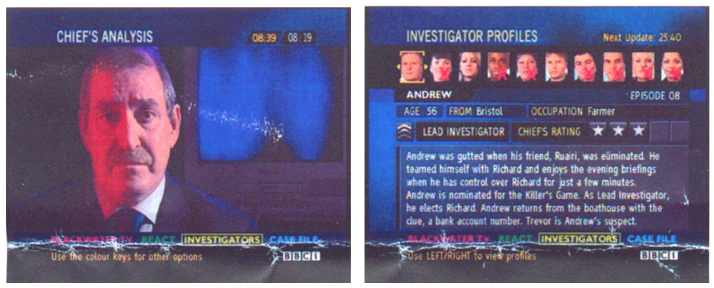
\includegraphics[width=1\textwidth]{images/MDDTIFFigure2.png}
	\caption{Viewing developments in The Murder Game}
	\label{fig:MDDTIFFigure2}
\end{figure}

\subsubsection{Problem}
Currently, each interactive application is bespoke. This greatly limits the number of programmes that can be accompanied by interactive content, as the applications are expensive to develop. The resulting UI is also different for different programmes, which is confusing to users. You are to design a system that will allow non-technical producers to build applications to accompany their programmes.

The application will sit on the right hand side of the screen (Figure \ref{fig:MDDTIFFigure3}), and display one of the following pieces of content:

\begin{itemize}
	\item A page of text, to be used for news stories, background information etc.
	\item A multiple choice vote, for example \emph{Man of the match} in a football match.
	\item A menu that allows the user to view items of content, including sub-menus.
\end{itemize}

The basic on-screen layout and navigational structure of the application has been defined by the user experience department, and producers are not able to change it.

\begin{figure}
	\centering
		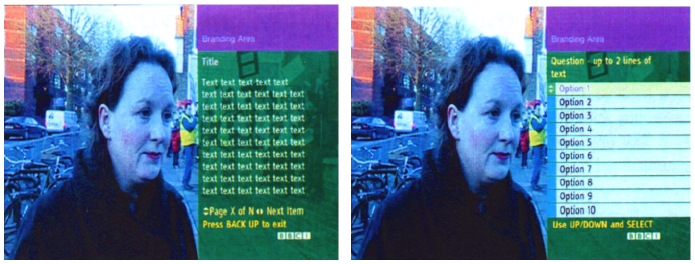
\includegraphics[width=1\textwidth]{images/MDDTIFFigure3.png}
	\caption{Different types of content}
	\label{fig:MDDTIFFigure3}
\end{figure}

\subsubsection{Use cases}
The following set of use cases emerged during discussions with the producers. They are ordered by their value to the producers, with the use case giving the most value first.

\paragraph{Case 1}
A producer would like to build an application for the soccer world cup finals, listing the teams and information about each, and allowing viewers to vote for the most likely winner.

\paragraph{Case 2}
As Case 1, but the teams should be listed by group (e.g. four teams in three groups). As the
teams are known before their division into groups by lots, it should be possible to define the
content for the teams first, and quickly add the structure of the groups, so that the application
can be running for users as soon as possible during the program that broadcasts the division
by lots.

\paragraph{Case 3}
A producer would like to use a page of text to provide analysis of the recent events in a rugby
match. A journalist with a laptop will need to change the text on the page throughout the
match. The user interface used by the journalist should not allow him to change the structure
of the whole application, only edit the text.

\paragraph{Case 4}
A producer has decided that the wording of a particular text page was better before the last
set of changes, and would like to revert it.

\subsubsection{Interactive application architecture}
Designing interactive applications requires relatively detailed knowledge of the standards for
each platform. For this reason, you should concentrate on the system used by producers to
define the application content, and its interfaces to black box components that build the
actual application. To define these interfaces, you will need some knowledge of the basic
architecture of interactive applications. The following crash-course should suffice.
Digital televisions contain a basic operating system, and a set of libraries providing functions
to display text and graphics, change the currently displayed video stream, etc. Applications
are designed and specified with a domain-specific modelling language (that you develop)
and delivered to digital televisions by inserting it as XML into the same broadcast stream that
contains the video and audio content. Once running, an application can be updated by
changing the XML in the broadcast stream. Applications can send reply messages to your
system, usually via a standard modem built into the television. Sending these reply messages
is very slow, and involves the viewer paying call charges. For these reasons, reply
messages can only be used for viewer initiated actions, such as responding to a vote.

\subsubsection{Code generation}
You should generate code like the following as plain text, rather than using any special
method for saving models as XML. This puts the various tools on an even footing, and
demonstrates the code generation facilities better for all kinds of code and other output files.
Handling white space and encodings is not vital, but the results should be machine and
human-readable.

\begin{lstlisting}[float=tbp, basicstyle=\ttfamily\footnotesize, flexiblecolumns=true, numbers=none, nolol=true, caption=Sample Generated XML, label=lst:MDDTIFXML, language=XML, tabsize=2]
<TVApp name=�World Cup 2010�>
	<Menu name=�World Cup�>
		<Vote name=�Who will win?�>
			<Choice name=�Estonia�/>
			<Choice name=�Lithuania�/>
		</Vote>
		<Text name=�World Cup trivia�>Trinidad &amp; 
			Tobago were the first ...</Text>
		<Menu name=�Teams�>
		�
		</Menu>
	</Menu>
</TVApp>
\end{lstlisting}


\subsection{Solution}

The case study presented above is within the scope of Epsilon as it involves a number of different model management tasks such as model validation, model-to-model transformation, model merging and model-to-text transformation. Moreover, to implement some cases (e.g. the code generation case), more than one individual model management tasks need to be combined. This section demonstrates an implementation of the functional requirements (cases) discussed above using Epsilon languages combined using the workflow mechanism presented in Chapter \ref{chp:Workflow}. The aim of this implementation is to cover as many cases as possible in an integrated manner with minimal duplication of code.

\subsubsection{Designing the TVApp DSL}

The first step of the solution is to design a Domain Specific Language (DSL) that enables users to design Interactive TV Applications. The TVApp DSL has been specified atop EMF by defining its abstract syntax in terms of ECore (using Emfatic \cite{Emfatic} as a convenience textual representation). A graphical overview of the DSL is presented in Figure \ref{fig:TVApps}.

\begin{figure}
	\centering
		%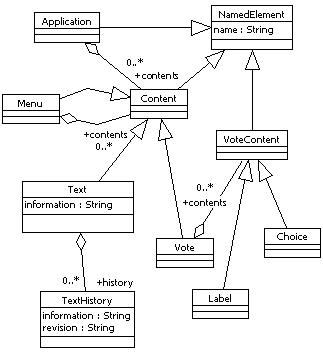
\includegraphics[width=0.45\textwidth]{images/TVApps}
		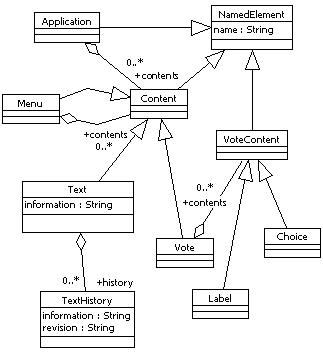
\includegraphics{images/TVApps}
	\caption{The TVApps Domain Specific Language}
	\label{fig:TVApps}
\end{figure}

\subsubsection{Generating a TVApp model for a Sports Competition}
\label{sec:Competition}

To address Case 1, a new Competition metamodel has been designed for capturing information about competitions, groups and participating teams. A graphical overview of the metamodel is displayed in Figure \ref{fig:Competition}. The design of the metamodel also satisfies the requirement of Case 2 for defining the team-related information first and then adding the teams into groups by modifying the \texttt{competitors} list of each group.

\begin{figure}
	\centering
		%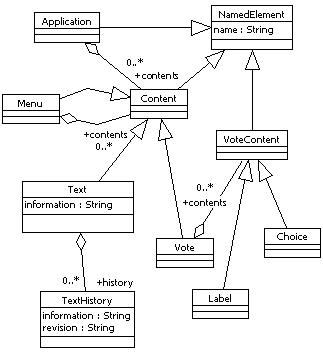
\includegraphics[width=0.45\textwidth]{images/TVApps}
		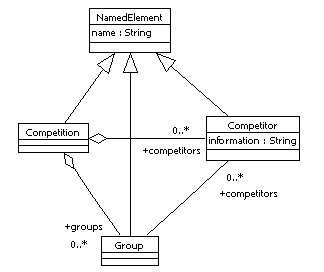
\includegraphics{images/Competition}
	\caption{The Competition Domain Specific Language}
	\label{fig:Competition}
\end{figure}

Before the Competition model can be transformed into a TVApp model, it should be validated against a number of constraints so that potential errors are detected at this level and not propagated to the TVApp model. In Listing \ref{lst:ValidateCompetition} an Epsilon Validation Language module is used for this purpose. The \emph{NameSpecified} constraint in line \ref{line:NameSpecified} specifies that all named elements (that is \emph{Groups} and \emph{Competitors}) must specify a non-empty name. Moreover, in line \ref{line:NotEmpty}, the \emph{NotEmpty} constraint applies to Groups and specifies that each group must have at least one competitor. Here it is worth noticing that in its guard, the \emph{NotEmpty} constraint requires that to apply to particular Group, the Group must first satisfy the \emph{NameSpecified} constraint presented above. Finally, in line \ref{line:InUniqueGroup}, the \emph{InUniqueGroup} constraint checks that each competitor only participates in one Group.

\begin{lstlisting}[basicstyle=\ttfamily\footnotesize, flexiblecolumns=true, numbers=left, nolol=true, caption=EVL module that validates a Competition model, label=lst:ValidateCompetition, language=EVL, tabsize=2]
context Competition!NamedElement {
	
	constraint NameSpecified { /*@\label{line:NameSpecified}@*/
		
		check : self.name.isDefined() and self.name.trim().length > 0
		
		message : self.eClass().name + " must provide a name"
		
	}
	
}

context Competition!Group {
	
	constraint NotEmpty { /*@\label{line:NotEmpty}@*/
		
		guard : self.satisfies("NameSpecified")
		
		check : self.competitors.size() > 0
		
		message : "Group " + self.name + " contains no competitors"
		
	}
	
}

context Competition!Competitor {
	
	constraint InUniqueGroup { /*@\label{line:InUniqueGroup}@*/
		
		guard : self.satisfies("NameSpecified")
		
		check : Competition!Group.allInstances.
			select(g|g.teams.includes(self)).size() <= 1
		
		message : "Competitor " + self.name + 
			" exists in more than one group."
	}
	
}
\end{lstlisting}

Having validated the input Competition mode, the Epsilon Transformation Language discussed in Section \ref{sec:ETL} is used to transform it into a TVApp model. The transformation displayed in Listing \ref{lst:TransformCompetition} defines that an \texttt{Application} and a \texttt{Vote} will be generated from each \texttt{Competition}, and that the \texttt{Vote} will contain a flattened sequence of \texttt{Label}s (one for each \texttt{Group}) and \texttt{Choice}s (one for each \texttt{Competitor} in the group).

\begin{lstlisting}[basicstyle=\ttfamily\footnotesize, nolol=true, flexiblecolumns=true, numbers=left, caption=ETL transformation that transforms a Competition model into a TVApp model, tabsize=2, label=lst:TransformCompetition, language=ETL]
rule Competition2Application
	transform c : Competition!Competition
	to a : TVApp!Application, v : TVApp!Vote {

	a.name = c.name + " Application";
	v.name = "Who will win the " + c.name + "?";	
	a.contents.add(v);
	
	for (g in c.groups) {
		v.contents.add(g.equivalent());
		for (memb in g.members) {
			v.contents.add(memb.equivalent());
		}
	}
}

rule Competitor2Choice
	transform co : Competition!Competitor
	to ch : TVApp!Choice {

	ch.name = co.name;
}

rule Group2Label
	transform g : Competition!Group
	to l : TVApp!Label {
	
	l.name = "Group " + g.name;
}
\end{lstlisting}

The two steps are combined into a composite task that validates and - if all constraints are satisfied - then transforms the Competition model using the workflow presented in Listing \ref{lst:TransformCompetitionWorkflow}. In lines \ref{line:LoadCompetitionTask} and \ref{line:LoadTVAppTask}, the involved models are loaded using the \emph{epsilon.loadModel} task. In line \ref{line:ValidateCompetitionTask} the Competition model is validated using the EVL module presented in Listing \ref{lst:ValidateCompetition}, and if all constraints are satisfied, in line \ref{line:TransformCompetitionTask}, it is transformed into a TVApp model using the ETL module presented in Listing \ref{lst:TransformCompetition}

\begin{lstlisting}[basicstyle=\ttfamily\footnotesize, flexiblecolumns=true, numbers=left, nolol=true, caption=Workflow that integrates the validation and transformation steps, label=lst:TransformCompetitionWorkflow, language=XML, tabsize=2]
<?xml version="1.0"?>
<project default="main">
	
	<epsilon.loadModel name="Competition" type="EMF"> /*@\label{line:LoadCompetitionTask}@*/
		<parameter name="modelFile" file="models/WorldCup.model"/>
		<parameter name="metamodelUri" value="CompetitionDsl"/>
		<parameter name="isMetamodelFileBased" value="false"/>
		<parameter name="readOnLoad" value="true"/>
	</epsilon.loadModel>
	
	<epsilon.loadModel name="TVApp" type="EMF"> /*@\label{line:LoadTVAppTask}@*/
		<parameter name="modelFile" file="models/TVApp3.model"/>
		<parameter name="metamodelUri" value="TVAppDsl"/>
		<parameter name="isMetamodelFileBased" value="false"/>
		<parameter name="readOnLoad" value="false"/>
	</epsilon.loadModel>

	<target name="main">

		<epsilon.evl src="ValidateCompetition.evl"> /*@\label{line:ValidateCompetitionTask}@*/
			<model ref="Competition"/>
		</epsilon.evl>		
		
		<epsilon.etl src="Competition2TVApp.etl"> /*@\label{line:TransformCompetitionTask}@*/
			<model ref="TVApp"/>
			<model ref="Competition"/>
		</epsilon.etl>
		
	</target>
	
</project>
\end{lstlisting}

\subsubsection{Integrating Live Reports}
\label{sec:LiveReports}

Case 3 requires that an external user must be able to update a particular text but not the structure of the application. To achieve this, the Report DSL presented in Figure \ref{fig:Report} has been designed. The rationale is that particular users can be only granted the permission to compose Report models which will then be used to automatically update the original application model via merging. To satisfy the requirement set in Case 4, when merging the original TVApp with a Report, the original information contained in the \texttt{Text}s which the Report updates is not lost but instead is stored in the form of a new \texttt{TextHistory} model element. The merge has been specified using the ECL and EML languages modules displayed in Listings \ref{lst:CaseStudyEML} and \ref{lst:CaseStudyECL} respectively. An alternative to designing the one-metaclass Report DSL would be to add the Report class to the existing TVApp DSL. However, it was deemed more appropriate with regard to modularity and separation of concerns to establish a new (albeit minimal) DSL instead.

\begin{figure}
	\centering
		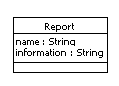
\includegraphics{images/Report}
	\caption{The Report Domain Specific Language}
	\label{fig:Report}
\end{figure}

As discussed in Section \ref{sec:EML}, EML operates in two steps. In the first step, correspondences are established between elements that need to be merged (using ECL or otherwise) and in the sequel corresponding elements are merged (using merge-rules) and non-matched elements are transformed into the target model (using transform-rules reused from ETL). In Listing \ref{lst:CaseStudyECL}, matching \texttt{Report}s from the Report model with \texttt{Text}s from an OldTVApp model is achieved through the \texttt{MatchReportWithText} ECL match-rule in line \ref{line:MatchReportWithText} that compares the names of the compared elements.

Then, in Listing \ref{lst:CaseStudyEML}, matching \texttt{Report}s and \texttt{Text}s are merged using the \texttt{MergeReportWithText} merge-rule in line \ref{line:MergeReportWithText} which specifies that the \texttt{Text} should be updated and that the old version of the text should be stored in the form of a new \texttt{TextHistory} model element with a proper information and revision number. The rest of the elements of the original TVApp model are copied to the target model using the transformation rules provided by the CopyTVApp module, displayed in Listing \ref{lst:CaseStudyCopyETL}, which is imported by the EML module using the \emph{import} statement in line \ref{line:ImportETL}.

\begin{lstlisting}[basicstyle=\ttfamily\footnotesize, flexiblecolumns=true, numbers=left, nolol=true, caption=ECL module that compares a TVApp with a Report model, label=lst:CaseStudyECL, language=ECL, tabsize=2]
rule MatchReportWithText /*@\label{line:MatchReportWithText}@*/
	match t : OldTVApp!Text
	with r : Report!Report {
	
	compare : r.name = t.name	
}
\end{lstlisting}

\begin{lstlisting}[basicstyle=\ttfamily\footnotesize, nolol=true, flexiblecolumns=true, caption=EML module that merges a TVApp with a Report model, tabsize=2, label=lst:CaseStudyEML, language=EML]
import "CopyTVApp.etl"; /*@\label{line:ImportETL}@*/

rule MergeReportWithText /*@\label{line:MergeReportWithText}@*/
	merge ot : OldTVApp!Text
	with r : Report!Report 
	into nt : NewTVApp!Text {
	
	nt.name = ot.name;
	nt.information = ot.information;
	nt.history ::= ot.history;
	
	var h : new NewTVApp!TextHistory;
	h.information = ot.information;
	h.revision = ot.history.collect(h|h.revision).max(0) + 1;
	nt.history.add(h);
	nt.information = r.information;
}
\end{lstlisting}

\begin{lstlisting}[basicstyle=\ttfamily\footnotesize, flexiblecolumns=true, numbers=left, nolol=true, caption=ETL transformation that copies a TVApp module, label=lst:CaseStudyCopyETL, language=ETL, tabsize=2]
rule CopyApplication
	transform s : OldTVApp!Application
	to t : Target!Application {
	
	t.name = s.name;
	t.contents ::= s.contents;
}
rule CopyText
	transform s : OldTVApp!Text
	to t : Target!Text {

	t.name = s.name;
	t.information = s.information;
	t.history ::= s.history;
}
rule CopyTextHistory
	transform s : OldTVApp!TextHistory
	to t : Target!TextHistory {

	t.revision = s.revision;
	t.information = s.information;
}
rule CopyVote
	transform s : OldTVApp!Vote
	to t : Target!Vote {

	t.name = s.name;
	t.contents ::= s.contents;
}
rule CopyChoice
	transform s : OldTVApp!Choice
	to t : Target!Choice {

	t.name = s.name;
}
rule CopyLabel
	transform s : OldTVApp!Label
	to t : Target!Label {

	t.name = s.name;
}
rule CopyMenu
	transform s : OldTVApp!Menu
	to t : Target!Menu {
	
	t.name = s.name;
	t.contents ::= s.contents;
}
\end{lstlisting}

In case a report in the Report model does not match a text in the TVApp model, the report is (correctly) not added into the target TVApp model. To inform the user about such cases, the EVL module of Listing \ref{lst:ValidateReport} is injected between the comparison and merging steps. The \emph{RefersToValidText} constraint specified in line \ref{line:RefersToValidText} examines the match-trace (\emph{trace}) established by the comparison step and requires that each report must match with a Text from the TVApp model.

\begin{lstlisting}[basicstyle=\ttfamily\footnotesize, flexiblecolumns=true, numbers=left, nolol=true, caption=EVL module that validates a Report model against a TVApp model, label=lst:ValidateReport, language=EVL, tabsize=2]
context Report!Report {
	
	constraint RefersToValidText { /*@\label{line:RefersToValidText}@*/
		
		check : trace.matches.exists(m|m.matching and m.right = self)
		
		message : "Report " + self.name + " refers to an undefined text"	
	}
}
\end{lstlisting}

The ECL, EVL and EML modules presented above are integrated using the workflow of Listing \ref{lst:CaseStudyMergingWorkflow}. In lines \ref{line:LoadReportTask}, \ref{line:LoadOldTVAppTask} and \ref{line:LoadNewTVAppTask} the involved models are loaded. In line 
\ref{line:MatchReportWithTVAppTask} the \emph{Report} model is compared with the \emph{OldTVApp} model using the ECL module of Listing \ref{lst:CaseStudyECL}

\begin{lstlisting}[basicstyle=\ttfamily\footnotesize, flexiblecolumns=true, numbers=left, nolol=true, caption=Workflow integrating the comparison\, validation and merging steps, label=lst:CaseStudyMergingWorkflow, language=XML, tabsize=2]
<?xml version="1.0"?>
<project default="main">
	
	<epsilon.loadModel name="Report" type="EMF"> /*@\label{line:LoadReportTask}@*/
		<parameter name="modelFile" file="models/Report.model"/>
		<parameter name="metamodelUri" value="ReportDsl"/>
		<parameter name="isMetamodelFileBased" value="false"/>
		<parameter name="readOnLoad" value="true"/>
	</epsilon.loadModel>
	
	<epsilon.loadModel name="OldTVApp" type="EMF"> /*@\label{line:LoadOldTVAppTask}@*/
		<parameter name="aliases" value="Source"/>
		<parameter name="modelFile" file="models/TVApp1.model"/>
		<parameter name="metamodelUri" value="TVAppDsl"/>
		<parameter name="isMetamodelFileBased" value="false"/>
		<parameter name="readOnLoad" value="true"/>
	</epsilon.loadModel>	
	
	<epsilon.loadModel name="NewTVApp" type="EMF"> /*@\label{line:LoadNewTVAppTask}@*/
		<parameter name="aliases" value="Target"/>
		<parameter name="modelFile" file="models/TVApp2.model"/>
		<parameter name="metamodelUri" value="TVAppDsl"/>
		<parameter name="isMetamodelFileBased" value="false"/>
		<parameter name="readOnLoad" value="false"/>
	</epsilon.loadModel>

	<target name="main">
		
		<epsilon.ecl src="MatchReportWithTVApp.ecl" 
			exportmatchtrace="trace"> /*@\label{line:MatchReportWithTVAppTask}@*/
			<model ref="OldTVApp"/>
			<model ref="Report"/>
		</epsilon.ecl>
		
		<epsilon.evl src="ValidateReport.evl"> /*@\label{line:ValidateReportTask}@*/
			<model ref="OldTVApp"/>
			<model ref="Report"/>
			<uses ref="trace"/>
		</epsilon.evl>
		
		<epsilon.eml src="MergeReportWithTVApp.eml" 
			usematchtrace="trace"> /*@\label{line:MergeReportWithTVAppTask}@*/
			<model ref="OldTVApp"/>
			<model ref="Report"/>
			<model ref="NewTVApp"/>
		</epsilon.eml>
		
		<epsilon.storeModel model="NewTVApp"/>
		
	</target>
	
</project>
\end{lstlisting}

\subsubsection{Generating XML from a TVApp model}
\label{sec:GeneratingXML}

To generate an XML document from a TVApp model, as required by the case study description, the intermediate XML metamodel displayed in Figure \ref{fig:XML} is used. Thus, the TVApp model is transformed into an XML model (Listing \ref{lst:TVApp2XML}) using the Epsilon Transformation Language, and then the textual representation of the XML model (Listing \ref{lst:EGL}) is generated using the Epsilon Generation Language. This approach promotes modularity and reuse by targeting XML-specific issues such as escaping and indentation in a separate transformation which can be reused as-is in other DSL to XML scenarios, and also complies with the requirement not to use a special (hard-coded) method for transforming XML models to text.

\clearpage

\begin{figure}
	\centering
		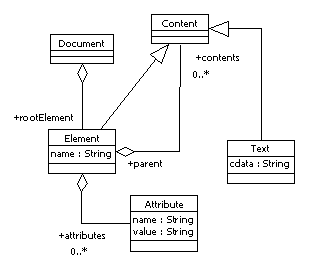
\includegraphics{images/XML}
	\caption{The XML Domain Specific Language}
	\label{fig:XML}
\end{figure}

\begin{lstlisting}[basicstyle=\ttfamily\footnotesize, nolol=true, flexiblecolumns=true, caption=ETL transformation that transforms TVApp models to XML models, tabsize=2, label=lst:TVApp2XML, language=ETL]
pre {
	var doc : new Xml!Document;
	doc.rootElement = TVApp!Application.
		allInstances.first().equivalent();
}

@abstract
rule NamedElement2Element
	transform ne : TVApp!NamedElement
	to n : Xml!Element {
	
	n.addAttribute("name", ne.name);
}

rule Application2Element
	transform a : TVApp!Application
	to n : Xml!Element extends NamedElement2Element{
	
	n.name = "Application";
	n.contents = a.contents.equivalent();
}

rule Vote2Element
	transform v : TVApp!Vote
	to n : Xml!Element extends NamedElement2Element {
	
	n.name = "Vote";	
	n.contents = v.contents.equivalent();
}

rule Choice2Element
	transform c : TVApp!Choice
	to n : Xml!Element extends NamedElement2Element {
	
	n.name = "Choice";	
}

rule Label2Element
	transform c : TVApp!Label
	to n : Xml!Element extends NamedElement2Element {
	
	n.name = "Label";
}

rule Text2Element
	transform t : TVApp!Text
	to e : Xml!Element extends NamedElement2Element {
	
	e.name = "Text";
	var text : new Xml!Text;
	text.cdata = t.information;
	e.contents.add(text);
}

rule Menu2Element
	transform m : TVApp!Menu
	to e : Xml!Element extends NamedElement2Element {
	
	e.name = "Menu";
	e.contents = m.contents.equivalent();
}

operation Xml!Element addAttribute
	(name : String, value : String) {
	var attr : new Xml!Attribute;
	attr.name = name;
	attr.value = value;
	self.attributes.add(attr);
}
\end{lstlisting}

The ETL transformation of Listing \ref{lst:TVApp2XML}, demonstrates two important characteristics of ETL: rule inheritance and state-changing operations. By inheriting from the abstract rule \textit{NamedElement2Element}, the rest of the rules are maintained simple and without duplication. Moreover, defining the \textit{addAttribute()} state-changing operation simplifies the \textit{NamedElement2Element} rule. 

\begin{lstlisting}[basicstyle=\ttfamily\footnotesize, nolol=true, flexiblecolumns=true, caption=EGL template that generates XML text from XML models, tabsize=2, label=lst:EGL, language=EOL]
<?xml version="1.0"?>
[%=Document.allInstances().first().rootElement.toString(0)%]

[%
operation Element toString(indent : Integer) : String {
	var str : String;
	str = indent.getIndent() + "<" + self.name.normalize();
	for (a in self.attributes) {
		str = str + " " + a.name.normalize() + 
			"='" + a.value.normalize() + "'";
		if (hasMore){
			str = str + " ";
		}
	}
	str = str + ">\r\n";
	for (c in self.contents) {
		str = str + c.toString(indent + 1);
	}
	str = str + indent.getIndent() + "</" + 
		self.name.normalize() + ">\r\n";
	return str;
}

operation Text toString(indent : Integer) : String {
	return (indent + 1).getIndent() + 
		self.cdata.normalize() + "\r\n";
}

operation Integer getIndent() : String {
	var indent : String;
	for (i in Sequence{1 .. self}){
		indent = indent + "  ";
	}
	return indent;
}

operation String normalize() {
	var normalized : String = self;
	if (not normalized.isDefined()) { 
		normalized = "";
	}
	else {
		normalized = normalized.replace("&", "&amp;");
		normalized = normalized.replace("<", "&lt;");
		normalized = normalized.replace(">", "&gt;");
		// etc
	}
	return normalized;
}
%]
\end{lstlisting}

Generating XML text from an XML model in Listing \ref{lst:EGL} involves much dynamic and little static text. Therefore, the vast majority of the serialization process is performed via string concatenation. By contrast, the header (processing instruction and comment) is only static text that is emitted as-is from the template.

\subsubsection{Integrating the Model-to-Model and the Model-to-Text steps}

To integrate the two steps presented above into a coherent process that transforms a TVApp model directly to textual XML, the Epsilon Workflow is used. Thus, in Listing \ref{lst:CaseStudyCodeGenWorkflow}, two tasks for loading the involved models (epsilon.loadModel), one that invokes the ETL transformation (epsilon.etl) and one that invokes the EGL model-to-text transformation on the intermediate XML model (epsilon.egl) are used.

\begin{lstlisting}[basicstyle=\ttfamily\footnotesize, nolol=true, numbers=left, flexiblecolumns=true, caption=The workflow that integrates the ETL and EGL tasks, tabsize=2, label=lst:CaseStudyCodeGenWorkflow, language=XML]
<?xml version="1.0"?>
<project default="main">
	
	<epsilon.loadModel name="TVApp" type="EMF">
		<parameter name="modelFile" file="models/ChampionsLeague.model"/>
		<parameter name="metamodelUri" value="TVAppDsl"/>
		<parameter name="isMetamodelFileBased" value="false"/>
		<parameter name="readOnLoad" value="true"/>
	</epsilon.loadModel>
	
	<epsilon.loadModel name="Xml" type="EMF">
		<parameter name="modelFile" file="models/TVAppXml.model"/>
		<parameter name="metamodelUri" value="Xml"/>
		<parameter name="isMetamodelFileBased" value="false"/> 
		<parameter name="readOnLoad" value="false"/>
	</epsilon.loadModel>

	<target name="main">

		<epsilon.etl src="TVApp2Xml.etl">
			<model ref="TVApp"/>
			<model ref="Xml"/>
		</epsilon.etl>
		
		<epsilon.egl src="Xml2Text.egl" target="output/TVApp.xml">
			<model ref="Xml"/>
		</epsilon.egl>
	</target>
</project>
\end{lstlisting}

\subsubsection{Generating a Mock-up of the TV Application}
\label{sec:Mockup}

A feature that is not required explicitly by the case study description, but which was regarded as particularly useful is to be able to \textit{preview} a TVApp model using a mock-up that closely resembles the appearance of the final deployed application. Therefore, EGL has been used to compose a model-to-text transformation that generates a set of linked HTML screens that emulate the look-and-feel and functionality of the deployed application. Listing \ref{lst:Mockup} presents the main template of the EGL solution that iterates the model and invokes the respective sub-templates (Text.egl, Menu.egl, Vote.egl) to generate the mockup HTML screens.

\begin{lstlisting}[basicstyle=\ttfamily\footnotesize, nolol=true, flexiblecolumns=true, caption=EGL template that generates mockup HTML screens for a TVApp model, tabsize=2, label=lst:Mockup, language=EOL]
[%
	import "include\\Common.eol";

	TemplateFactory.setTemplateRoot("workspace\\MDD-TIF");
	TemplateFactory.setOutputRoot("workspace\\MDD-TIF\\html");
	
	var header : Template = 
		TemplateFactory.load("include\\Header.egl");
	var text : Template = 
		TemplateFactory.load("include\\Text.egl");	
	var menu : Template = 
		TemplateFactory.load("include\\Menu.egl");
	var vote : Template = 
		TemplateFactory.load("include\\Vote.egl");
	var footer : Template = 
		TemplateFactory.load("include\\Footer.egl");
	
	var contents : String = "default";
	
	if (Application.isType(content) or Menu.isType(content)) {
		menu.populate("menu", content);
		contents = menu.process();
		
		// Recursively generate the pages 
		// for the contents of this
		// application / menu
		for (child in content.contents) {
			var page : Template = TemplateFactory.load("Page.egl");
		
			page.populate("content", child);
			
			page.generate(child.filename());
		}

	} else {
		if (Text.isType(content)) {
			text.populate("text", content);
			contents = text.process();

		} else {
			if (Vote.isType(content)) {
				vote.populate("vote", content);
				contents = vote.process();
			}
		}
	}
	
%]
[%=header.process()%]
[%=contents%]
[%=footer.process()%]
\end{lstlisting}

%\subsection{Other Submitted Solutions}

%Is this worth writing?

\subsection{Summary}

The case study presented in this section involves four different model management tasks, three of which comprise of more than one step, for each of which a different model management language is more appropriate. Table \ref{tab:CaseStudyMatrix} provides an overview of the tasks and the languages involved in providing a solution for each one.

\begin{table}
	\centering
		\begin{tabular}{|l|l|l|}\hline
			\textbf{Task} & \textbf{Languages used} \\\hline
			Transform a Competition into a TVApp model & EVL, ETL \\\hline
			Provide Support for Live Reports & ECL, EVL, EML \\\hline
			Generate XML from a TVApp model & ETL, EOL \\\hline
			Generate Mock-up screens from a TVApp model & EGL \\\hline
		\end{tabular}
	\caption{Matrix of Tasks and applied Languages}
	\label{tab:CaseStudyMatrix}
\end{table}

The solution has demonstrated that the layered architecture proposed in this work enables users to decompose complex tasks into steps that are easily manageable with one of the task-specific languages provided and then exploit the inherent interoperability of the individual languages to compose the steps into coherent composite tasks using the proposed workflow solution.